\chapter{Warning Message Design}
\label{Design}

This study involves participants reacting to different simulated warning messages of varying severity levels (mild, medium, and high severity) as well as the browser's default warnings as a control. We designed several warning messages for these conditions. The same warning structure is used in all cases, with warning content and style altered to reflect the risk of various simulated malicious situations. By experimenting with the severity levels (and thus the warning message features), we will examine how impressions and behaviour toward the different messages compare to one another.

The study aims to assess which aspects of warning messages more strongly convey severity and risk to users, and whether or not altering the expressed level of severity impacts user adherence (and by how much). As such, it is important to convey this notion of severity effectively through the messages' visuals so that users are able to quickly and intuitively distinguish between them -- even having never seen them before. Our warning messages utilize colour, wording, and imagery as cues for severity, which we hypothesize will increase understanding by maximizing the number of ways in which the danger level can be inferred.

\begin{figure}[th]
	\centering
	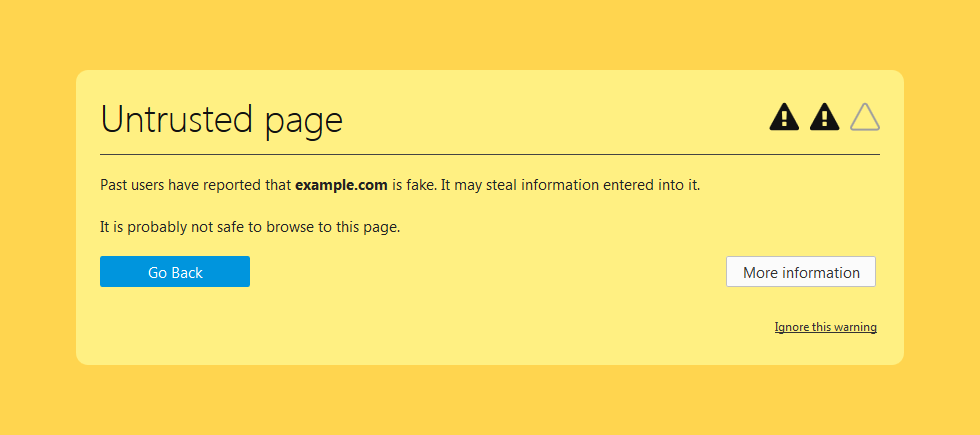
\includegraphics[width=\textwidth]{Figures/Warning-Medium-Phishing}
	\decoRule
	\caption[Medium severity phishing warning]{A medium severity phishing warning. Note the yellow colour, cautious wording, and two triangular icons. Colours, imagery, and wording are made more/less strict and intense as severity increases/decreases.}
	\label{fig:Warning-Medium-Phishing}
\end{figure}

\section{Colour}
Making colour the largest element is a reasonable design decision and is supported by research by Braun et al. \cite{braun1994color}, which indicates that colour plays an important role in warning adherence. In their study, participants complied with red warnings more frequently due to a higher associated likelihood of harm.

A message's colour covers the entire page, making it its largest, most obvious element. For our tiered warnings we chose to use colours with common real-world associations so their meanings would be intuitive, hopefully reducing the time and cognitive load needed to interpret the meaning of a given message.

Grey was chosen for low severity messages as it is usually considered neutral and is similar to the default background colour of a new tab in the browser. Yellow was used for medium severity messages due to its widespread association with ``caution'' (e.g., traffic lights, caution tape, construction). Red was employed in high severity messages because of its common link to stopping and danger (e.g., traffic lights, real-life warning signs, some existing browser warnings).

\section{Body Text}
Past studies have found that users are unlikely to read technical jargon or large amounts of text \cite{almuhimedi2014reputation, bravo2011bridging}. It is therefore important to convey a message's severity in an easy to understand manner while remaining concise. Our tiered warnings feature four main textual elements to accomplish this: the title, final note, threat explanation, and ``more information'' text.

\subsection{Title and Final Note}
The title and final note are modified based solely on a warning's severity (and not its type). They serve as global indicators of severity. The title of the warning aims to summarize the severity of the situation in two or three words. The final note serves as a cautionary message, further aiding in conveying the severity to the user by leaving them with some notion of how to proceed. See table \ref{tab:Tiered-Text} for these strings.

{\renewcommand{\arraystretch}{1.2}
\begin{table}[!htb]
	\small
	\centering
	\begin{tabularx}{0.85\textwidth}{|l|X|X|}
		\hline
		\textbf{Severity} & \textbf{Title} & \textbf{Final Note}\\
		\hline
		Low 	& Suspicious page 				& This page may be dangerous. Proceed with caution\\
		\hline
		Medium 	& Untrusted page 				& It is probably not safe to go to this page\\
		\hline
		High 	& Potential threat detected! 	& \textbf{It is highly recommended that you do not continue}\\
		\hline
	\end{tabularx}
	\caption{Tiered warning titles and final notes}
	\label{tab:Tiered-Text}
\end{table}}

\subsection{Threat Explanation}
Four different types of warnings were used for the study: SSL, malware, phishing, and unwanted software. For each type, a different group of threat descriptions was used. The purpose of this text is to emphasize the potential threat a user may be exposed to by visiting the page, as well as its impact. More stress and greater detail are given as the severity increases, with high severity warnings offering real-world examples of what can happen (e.g., passwords and financial information being stolen). The explanations are listed below in table \ref{tab:Tiered-Body}.

{\renewcommand{\arraystretch}{1.2}
\begin{table}[!htb]
	\small
	\centering
	\begin{tabularx}{\textwidth}{|l|X|X|X|X|}
		\hline
		\textbf{Severity} & \textbf{SSL} & \textbf{Malware} & \textbf{Phishing} & \textbf{Unwanted S/W}\\
		& \textbf{Warning} & \textbf{Warning} & \textbf{Warning} & \textbf{Warning}\\
		\hline
		Low
		& The authenticity of example.com, and thus its security, was unable to be verified.
		& example.com may contain software which can harm your computer.
		& The identity of the page at example.com, and thus the source of its contents, could not be verified.
		& example.com may contain potentially misleading and deceptive software\\
		\hline
		Medium
		& The identity of example.com could not be confirmed and therefore its security cannot be guaranteed. Information sent may be visible to others.
		& example.com may contain software which can harm your computer.
		& Past users have reported that example.com is fake. It may steal information entered into it.
		& Users have reported that example.com contains potentially unwanted software which it tries to install.\\
		\hline
		High
		& A secure connection could not be established to example.com. While browsing this website, it is possible for an attacker to monitor your activity and steal your personal information (passwords, financial information, conversations, etc.).
		& example.com has been reported by users in the past as being dangerous. It could contain malware.
		& example.com has been reported by users and it is likely impersonating another page. Any personal information entered (passwords, financial information, conversations, etc.) could be stolen.
		& example.com contains potentially dangerous and unwanted software which can negatively impact your computer. Users have reported that the page also employs trickery to encourage downloads of this software (e.g., fake download buttons).\\
		\hline
	\end{tabularx}
	\caption{Tiered explanations of threats}
	\label{tab:Tiered-Body}
\end{table}}

\subsection{``More Information'' Text}
It is presumed that users who click the ``more information'' button are seeking a detailed explanation. As such, the text revealed when the button is clicked is more verbose than the threat explanation, and remains the same for every tier of message of the same warning type (see table \ref{tab:Tiered-More-Info}). This always gives inquisitive users the level of detail they are seeking. The text is still relatively short and devoid of overly-technical wording.

{\renewcommand{\arraystretch}{1.2}
\begin{table}[!htb]
	\small
	\centering
	\begin{tabularx}{\textwidth}{|X|X|X|X|}
		\hline
		\textbf{SSL} & \textbf{Malware} & \textbf{Phishing} & \textbf{Unwanted S/W}\\
		\textbf{Information} & \textbf{Information} & \textbf{Information} & \textbf{Information}\\
		\hline
		Secure websites identify themselves using certificates. When a certificate is unable to be verified, it can mean that security settings have been misconfigured, security of the website has been compromised, or that an attacker is impersonating the website. In any case, any personal information entered into the page is at risk of being seen by others (e.g., passwords and credit card numbers).
		& Pages containing harmful software (malware) attempt to infect and take over your web browser and computer by installing malicious applications. Such software can allow attackers to steal personal information, delete files, and infect others.
		& Imitation pages impersonate sources you may trust and allow criminals to steal sensitive information such as passwords and credit card numbers. These pages may look and behave as expected, however information entered into them is actually sent to a criminal - not the organization the page claims to represent.
		& Unwanted software is classified as software that may behave in ways that you do not approve of or are not aware of. Examples include adware and spyware. Such software may also attempt to install additional unwanted software without your consent. Pages that distribute unwanted software often encourage downloads through deception (e.g., fake links, fake download buttons, and fake exit buttons).\\
		\hline
	\end{tabularx}
	\caption{Tiered warning ``more information'' text}
	\label{tab:Tiered-More-Info}
\end{table}}

\section{Imagery}
Our tiered messages feature a number of triangular ``warning'' icons alongside the title, with the number indicating severity (ranging from one icon for low severity to three icons for high severity). An example can be seen in figure \ref{fig:Warning-Medium-Phishing}. They are composed of an exclamation mark inside of a triangle -- an image often used on cautionary signs. The intent of this visual indicator is to provide a quick way for users to assess the severity of warnings. It is our hope that it will be useful in addition to the rest of the message, as well as on its own as a quick gauge of severity for users who do not read the message.
